\section{Introducción}
\par{Este trabajo propone observar las diferencias en los tiempos de cómputo debidas al aprovechamiento del modelo de procesamiento SIMD con respecto a implementaciones en C.}
\par{Se implementaron diversos filtros de los cuales se expone una breve explicación a continuación y luego se detallan en sus respectivas secciones.}
\begin{itemize}
\item[•] \textbf{Smalltiles:} genera una imagen del mismo tamaño de la original que la contiene 4 veces, una en cada cuadrante.
\item[•] \textbf{Rotar canales:} intercambia los colores de modo que lo azul pasa a ser rojo, lo rojo, verde y lo verde, azul.
\item[•] \textbf{Pixelar:} como su nombre lo indica, pixela la imagen disminuyendo la definición.
\item[•] \textbf{Combinar:} consiste en combinar 2 imágenes en función de un parámetro.
\item[•] \textbf{Colorizar:} intensifica los colores predominantes en cada píxel.
\end{itemize}

\begin{center}
 \begin{tabular}{cccc}
   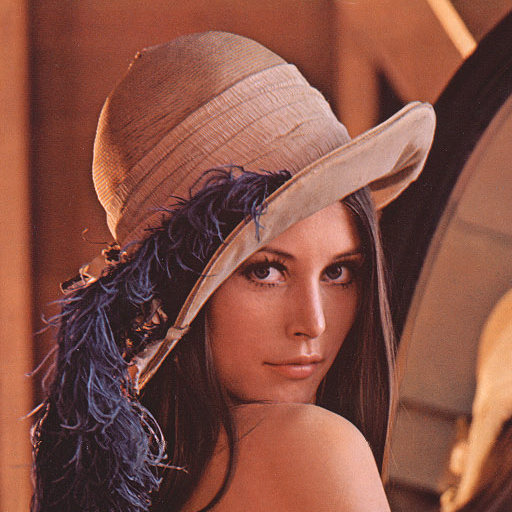
\includegraphics[width=0.2\textwidth]{imagenes/lena.png} &
   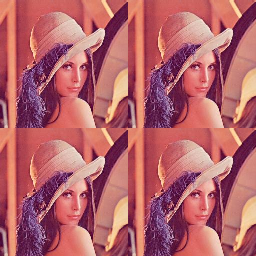
\includegraphics[width=0.2\textwidth]{imagenes/lena-smalltiles.png} &
   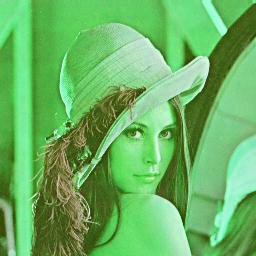
\includegraphics[width=0.2\textwidth]{imagenes/lena-rotar-canales.png} \\
   Imagen original & Smalltiles & Rotar \\
   \\
   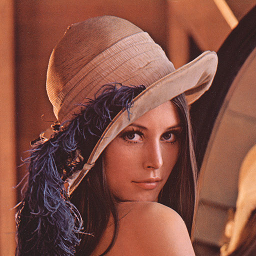
\includegraphics[width=0.2\textwidth]{imagenes/lena-pixelar.png} &
   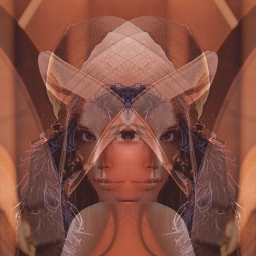
\includegraphics[width=0.2\textwidth]{imagenes/lena-combinar.png} &
   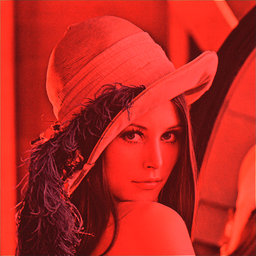
\includegraphics[width=0.2\textwidth]{imagenes/lena-colorizar.png} \\
   Pixelar & Combinar & Colorizar \\
 \end{tabular}
\end{center}

\par{Además de implementar los filtros en C y en Assembler se llevaron a cabo distintos experimentos para confirmar la hipótesis que motivó el trabajo, el hecho de que el procesamiento SIMD es más eficiente y permite resultados mucho más veloces que los obtenidos con las implementaciones de C.}

\subsection{Experimentacion}
\par{En nuestra experimentación elegimos testear los tiempos de ejecución de nuestros algoritmos corriendo cada implementación una cantidad fija de veces y luego, en el caso de los gráficos de barras, nos quedamos con el promedio y también ploteamos el desvío estandar. En el resto de los gráficos siempre nos quedamos con el mínimo valor obtenido, ya que creemos que este representa una corrida donde el procesador intervino lo menos posible.}